\documentclass[a4paper,10pt]{article}
\usepackage[utf8]{inputenc}
\usepackage{lmodern}
\usepackage[T1]{fontenc}
\usepackage[italian]{babel}

\usepackage{amsmath}
\usepackage{amsfonts}
\usepackage{amssymb}

\usepackage{graphicx}
\usepackage[dvipsnames]{xcolor}  %colori

\usepackage{pgf}
\usepackage{tikz}
\usetikzlibrary{arrows,shapes,snakes,automata,backgrounds,petri}	% Finite States Machine

\usepackage[left=2cm,right=2cm,top=2cm,bottom=2cm]{geometry}
\geometry{a4paper}
\setlength\marginparwidth{40pt}
\setlength\marginparsep{1pt}

\usepackage{verbatim}
\usepackage{lipsum}

\usepackage{booktabs}
\usepackage{subfig}
\usepackage{float}
\usepackage{wrapfig}

\usepackage[colorlinks=true, linkcolor=black, urlcolor=blue, citecolor=darkgray, filecolor=darkgray]{hyperref}   %per gli hyperlink
\usepackage[italian, sort, noabbrev, capitalise]{cleveref}
\usepackage[bottom]{footmisc}

\usepackage[cdot, thickqspace, squaren]{SIunits}
% macro
\def\code#1{\texttt{#1}}

\title{Esercitazione 15: Misura della costante di Boltzmann attraverso misure di rumore}
\author{Gruppo BL \\ Candido Alessandro, Luzio Andrea, Mazziotti Fabrizio}

\begin{document}

\maketitle

\section{Scopo e Strumentazione}
In questa esercitazione si vuole effettuare una misura della costante di Boltzmann attraverso la
misura del rumore termico in una serie di resistenze con valori diversi.

\noindent La strumentazione è quella solitamente presente sul banco di lavoro, e inoltre si è usato:
\begin{itemize}
	\item INA114: Precision instrumentation amplifier;
	\item AD708: ultra low offset dual op-amp (2 integrati);
	\item AD736: true rms-to-dc converter.
\end{itemize}

\subsubsection*{Schema complessivo}

Lo schema a blocchi del circuito è riportato in \cref{fig:blocks}.

\begin{figure}[H]
	\centering
	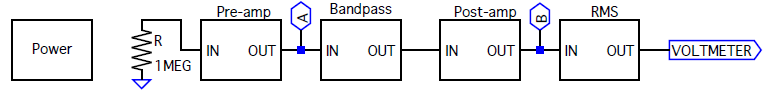
\includegraphics[width=\textwidth]{../grafici/Blocks.png}
	\vspace*{10pt}
	\caption{Schema a blocchi del circuito complessivo.}
	\label{fig:blocks}
\end{figure}

\begin{wrapfigure}[11]{R}{0.4\textwidth}
	\vspace{-10pt}
	\centering
	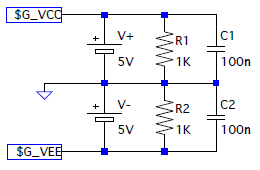
\includegraphics[width=0.4\textwidth]{../grafici/Filter.png}
	\vspace{-6pt}
	\caption{Schema di filtraggio per le alimentazioni.}
	\label{fig:powfilter}
	\vspace{-12pt}
\end{wrapfigure}

Si sono fissate le alimentazioni a $\sim \unit{5}{\volt}$ e si è montatp fra esse lo shcema di filtraggio riportato in  \cref{fig:powfilter}.

Si è proceduto con il montaggio dei singoli blocchi di circuito, che verranno illustrati individualmente nella prossima sezione.


\section{Implementazione dei blocchi di circuito}

\subsection{Pre-amplificatore}

Si è montato il circuito in \cref{fig:preamp} costituito da due amplificatori: il primo è l'integrato INA114 il cui guadagno atteso è pari a $A_0 = (1+ 50k\Omega/R_1) = 51.6 \pm 0.5$; %, dove la resistenza da 50 k$\Omega$ è il stata presa nominale poichè risultato delle resistenze interne all'integrato.


% la resistenza da 1k l'abbiamo misurata, quella da 50k sarà il risultato delle resistenze che stanno dentro all'integrato, che mettiamo nominale?

il secondo è costituito da un opamp con feedback sull'ingresso invertente. Il guadagno atteso di questa seconda parte di circuito è dato da $A_1 = R_3/R_2 = 14.4 \pm 0.2 $.

\begin{wrapfigure}{L}{0.6\textwidth}
	\vspace{-10pt}
	\centering
	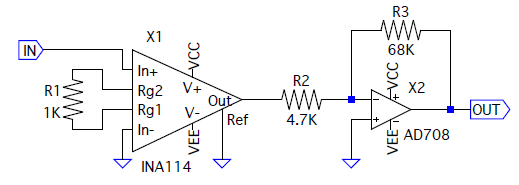
\includegraphics[width=0.6\textwidth]{../grafici/PreAmp.png}
	\vspace{-12pt}
	\caption{Schema del circuito: pre-amplificatore.}
	\label{fig:preamp}
	\vspace{-6pt}
\end{wrapfigure}


Le resistenze utilizzate sono riportate in \cref{tab:resistenze}.

\begin{table}[H]
	\centering
	\begin{tabular}{ccc}
		\hline
		$R_1[\Omega]$ & $R_2[k\Omega]$ & $R_3[k\Omega]$\\
		\hline
		$989\pm9$ & $4.71\pm0.05$ & $67.9\pm0.6$\\
		\hline
	\end{tabular}
	\caption{Resistenze utilizzate nel circuito in \cref{fig:preamp}.}
	\label{tab:resistenze}
\end{table}




\subsubsection*{Amplificazione \\e risposta in frequenza}

In primo luogo si è misurata la risposta in frequenza del solo amplificatore INA staccando la seconda parte del circuito e mandando al suo ingresso un'onda sinusoidale dal generatore di funzioni%con ampiezza picco-picco di $V_pp = 9.4\pm 0.2 mV$. 
Come funzione modello si è scelto di prendere quella per un generico passa-basso:
\begin{equation}
\frac{A_0}{\sqrt[]{1+(\frac{f}{f_{t,0}})^2}}
\end{equation}
Le misure prese ed il fit sono riportati rispettivamente in \cref{??} e in \cref{fig:prepreamp}.

TABELLA


\begin{figure}[H]
	\centering
	\includegraphics[width=0.7\textwidth]{../grafici/prepreamp.pdf}
	\caption{Risposta in frequenza dell'amplificatore INA.}
	\label{fig:prepreamp}
\end{figure}


Dal fit si ottengono come risultati $A_0 = $, $f_t,0 = $, $\chi^2/DOF = /$. Il guadagno è in buon accordo con quanto atteso. 
CHI2

In secondo luogo si è mandata un'onda sinusoidale all'ingresso della seconda parte del circuito (prima della resistenza $R_2$) e si è studiata la sua risposta in frequenza.
Anche in questo caso come funzione modello si è scelto di prendere quella per un generico passa-basso:
\begin{equation}
\frac{A_1}{\sqrt[]{1+(\frac{f}{f_{t,1}})^2}}
\end{equation}
 Le misure prese ed il fit sono riportati rispettivamente in \cref{??} e in \cref{fig:postpreamp}.

TABELLA


\begin{figure}[H]
	\centering
	\includegraphics[width=0.7\textwidth]{../grafici/postpreamp.pdf}
	\caption{Risposta in frequenza del secondo amplificatore.}
	\label{fig:postpreamp}
\end{figure}

Dal fit si ottengono come risultati $A_1 = $, $f_t,1 = $, $\chi^2/DOF = /$. Il guadagno è in buon accordo con quanto atteso. 
CHI2

Inoltre affinché il circuito amplifichi il segnale al massimo possibile (quindi con l'amplificazione ricavata), è necessario che le frequenze di taglio ottenute nei due casi risultino maggiori della frequenza di risonanza del filtro passabanda (vedi prossima sezione), che è attesa essere $\sim$ 6-7 kHz. In entrambi i casi ciò è rispettato.






\subsection{Filtro passabanda e post-amplificatore}

\begin{wrapfigure}{R}{0.5\textwidth}
	\vspace{-10pt}
	\centering
	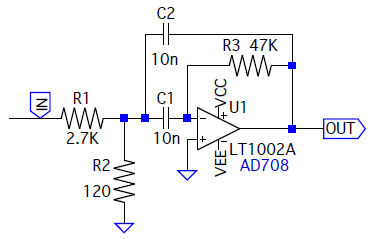
\includegraphics[width=0.5\textwidth]{../grafici/Bandpass.png}
	\vspace{-12pt}
	\caption{Schema del circuito: filtro passabanda.}
	\label{fig:powamp}
	\vspace{-6pt}
\end{wrapfigure}



\begin{wrapfigure}{L}{0.6\textwidth}
	\vspace{-10pt}
	\centering
	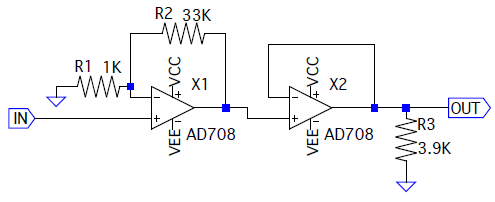
\includegraphics[width=0.6\textwidth]{../grafici/PostAmp.png}
	\vspace{-12pt}
	\caption{Schema del circuito: post-amplificatore.}
	\label{fig:powamp}
	\vspace{-6pt}
\end{wrapfigure}




\subsubsection*{Amplificazione e risposta in frequenza}

Si è misurata l'amplificazione e la risposta in frequenza dei due circuiti congiuntamente. Naturalmente il contributo maggiore alla risposta in frequenza sarà quello del passabanda, poiché gli op-amp del post-amplificatore hann un comportamento ideale fino a frequenze abbastanza elevate (molto maggiori dei $\sim 6 \kilo\hertz $ della frequenza centrale).

Si riportano in \cref{fig:bandpass} i dati presi per la risposta in frequenza e il fit che si è fatto di essi (il grafico su cui sono mostrati è bilogaritmico).
La funzione di cui stato eseguito il fit è:
\[ A(f) = A_2^\star \frac{f}{\sqrt{(f^2-f_0^2)^2 + \left(\frac{f_0 f}{Q}\right)^2}} \]

e i parametri trovati dal fit sono:
\[ A_2^\star=(1.495 \pm 0.012)\cdot10^5 \qquad Q=57.6 \pm 1.9 \qquad f_0=6.084 \pm 0.007 \kilo\hertz  \]
da cui si può dedurre il valore dell'amplificazione di centro banda $ A_{2,0} $ e la larghezza di banda $ \Delta f $:

\begin{figure}[H]
	\centering
	\includegraphics[width=0.7\textwidth]{../grafici/passabanda.pdf}
	\vspace*{10pt}
	\caption{Amplificazione e risposta in frequenza degli stadi passabanda e post-amplificatore in serie.}
	\label{fig:bandpass}
\end{figure}

\subsection{Convertitore RMS}

\begin{wrapfigure}{L}{0.4\textwidth}
	\vspace{-10pt}
	\centering
	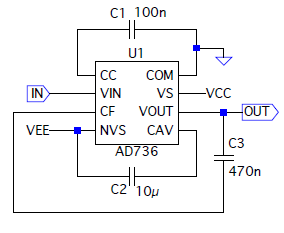
\includegraphics[width=0.4\textwidth]{../grafici/RMSconverter.png}
	\vspace{-12pt}
	\caption{Schema del circuito: convertitore RMS.}
	\label{fig:powamp}
	\vspace{-6pt}
\end{wrapfigure}



\subsubsection*{Calibrazione}



\begin{figure}[H]
	\centering
	\includegraphics[width=0.7\textwidth]{../grafici/calibrazione.pdf}
	\vspace*{10pt}
	\caption{Fit della calibrazione del convertitore RMS.}
	\label{fig:blocks}
\end{figure}

\section{Misura della costante di Boltzmann}
Si sono montati i vari circuiti tutti insieme, come schematizzato dalla \cref{fig:blocks}. Si è misurato il valore $V_{RMS}$ in uscita al circuito al variare della resistenza in ingresso. Per ogni resistenza sono stati presi più valori di $V_{RMS}$ poiché la misura oscillava molto. Si è poi effettuata una media dei valori presi. I dati ottenuti sono riportati in \cref{tab:lastfit}.

\begin{table}[H]
	\centering
	\begin{tabular}{cccc}
		\hline
R[k$\Omega$] & $\delta$ R [k$\Omega$] & $V_{RMS}[mV]$  & $\delta$ $V_{RMS}[mV]$ \\
\hline
0.985 & 0.009 & 35 & 1 \\
1.18 & 0.01 & 36.1 & 0.5 \\
1.48 & 0.01 & 36.7 & 0.8 \\
2.14 & 0.03 & 37.5 & 0.6 \\
3.26 & 0.04 & 38.9 & 0.7 \\
3.83 & 0.04 & 41.3 & 0.9 \\
4.68 & 0.05 & 43.9 & 0.9 \\
5.59 & 0.05 & 46.7 & 0.8 \\
6.71 & 0.06 & 50.3 & 0.8 \\
8.11 & 0.07 & 51.1 & 0.8 \\
9.91 & 0.09 & 54 & 1 \\
9.97 & 0.08 & 58 & 2 \\
11.8 & 0.1 & 62 & 2 \\
17.9 & 0.2 & 72 & 2 \\
		\hline
	\end{tabular}
	\caption{Valori delle resistenze utilizzate e del potenziale all'uscita del circuito.}
	\label{tab:lastfit}
\end{table}

Le relazioni attese che legano $V_{RMS}$, le resistenze utilizzate, i guadagni ottenuti e la costante di Boltzmann $k_b$ sono le seguenti:

\begin{equation}
V_{RMS} = V_{0n} \sqrt[]{1+\frac{R}{R_T}+\frac{R^2}{R_n ^2}}
\label{fitt}
\end{equation}
dove R è la resistenza in ingresso, $R_T, V_0n e R_n$ sono parametri che si otterranno dal fit a questa funzione.

\begin{equation}
V_0n = A V_n
\label{resnull}
\end{equation}
 che rappresenta il rumore in uscita a resistenza nulla. Il Guadagno $A$ è quello complessivo di tutto il circuito, cioè $A = A_0 A_1 A_2 A_3 = (1.17\pm0.02)e+05 $.
 
 \begin{equation}
 R_T = \frac{V_n^2}{4k_b T \Delta f} = \frac{V_0n^2}{4k_b A_0 T \Delta f}
 \label{kb}
 \end{equation}
  che è la resistenza equivalente del rumore serie dell'amplificatore riferito all'ingresso.

Si è quindi effettuato un fit alla $\eqref{fitt}$ ottenendo come risultati $V_0n = 0.0329\pm0.0007 V$ , $R_T = (7\pm1)e+03 \Omega $, $R_n = (1.5+/-0.2)e+04 \Omega$, $\chi ^2 /DOF$ = 93/11. Il $\chi ^2$ risulta essere leggermente alto; si ritiene che ciò sia dovuto ad una sottostima degli errori.
%... lascio così come commento? chi2 senza media = 17.

Il grafico è mostrato in \cref{fig:lastfit}.


\begin{figure}[H]
	\centering
	\includegraphics[width=0.7\textwidth]{../grafici/lastfit.pdf}
	\caption{Fit di $V_{RMS}$ in funzione di R.}
	\label{fig:lastfit}
\end{figure}



\subsection{Stima diretta dell'amplificazione \\e risposta in frequenza del circuito complessivo}
Si è misurata direttamente l'amplificazione e la risposta in frequenza del circuito complessivo mandando segnali molti piccoli in ingresso utilizzando un partitore 1000:1 (si sono utilizzate a tal proposito le resistenze $R_1 = 9.91\pm0.09 k\Omega $ e $R_2 = 10.1\pm0.4 \Omega$).
I dati raccolti sono mostrati in \cref{tab:partit}.

\begin{table}[H]
	\centering
	\begin{tabular}{cccc}
		\hline
a&b&b&FINIRE\\
		\hline
	\end{tabular}
	\caption{Valori delle frequenze utilizzate e del potenziale in uscita al circuito utilizzando un partitore 1000:1}
	\label{tab:partit}
\end{table}

Si è effettuato un fit su questi dati per trovare l'amplificazione complessiva del circuito. Si è modellizzato tutto il circuito come se fosse un unico passabanda amplificato, con amplificatori ideali (con frequenza di taglio costante). La funzione di fit è la seguente:
\begin{equation}
\frac{1}{\sqrt[]{1+(\frac{f}{f_t})^2}} \frac{A f}{\sqrt[]{(f - f_0)^2+ \frac{f^2 f_0^2}{Q} )}} 
\end{equation}

Questa stima potrebbe ulteriormente essere migliorata utilizzando come modello il prodotto tra le varie funzioni di trasferimento degli amplificatori (tutti con frequenze di taglio diverse) e il passabanda, ma come si può notare dal fit e dai suoi risultati, anche il modello utilizzato è fitta bene i dati. Il grafico è mostrato in \cref{fig:ampltot} e i risultati in \cref{tab:risult}.

\begin{figure}[H]
	\centering
	\includegraphics[width=0.7\textwidth]{../grafici/amp_alternativa_imp.pdf}
	\caption{fit dell'amplificazione totale in funzione della frequenza del segnale in ingresso al circuito.}
	\label{fig:ampltot}
\end{figure}

\begin{table}[H]
	\centering
	\begin{tabular}{ccccc}
		\hline
A & Q & $f_0[Hz]$ & $f_t[Hz]$ & $\chi^2/DOF$ \\
(1.57$\pm$0.06)e+08 & 9.0$\pm$0.4 & 6794$\pm$35 & (9.1$\pm$0.8)e+03 & 16/19 \\
\hline
	\end{tabular}
	\caption{Risultati del fit per valutare l'amplificazione complessiva del circuito e la sua risposta in frequenza.}
	\label{tab:risult}
\end{table}

I valori ottenuti per l'amplificazione totale e per la banda passante sono rispettivamente A = (4.84$\pm$0.08)e+04 e $\Delta f$ = (4.75$\pm$0.23)e+03 Hz.

%non sono sicuro dei risultati che ho messo soprattutto delta f che esce 3 ordini di grandezza diversa, per piacere controllate ed aggiustate.


\subsection{Risultati finali}
A questo punto, utilizzando la \eqref{resnull} e la \eqref{kb} si è ricavata la costante di Boltzmann con entrambi i metodi sopra descritti. Si sono ottenuti come risultati rispettivamente $k_b = (1.44\pm0.19)e-23 J/K$ e $k_{b,1000:1} = (1.17\pm0.16)e-23 J/K $. Il valore atteso per la costante di Boltzmann è $k_b$ = 1.380e-23 J/K. I risultati ottenuti sono entrambi compatibili con il valore atteso. 


\end{document}